% *********************************************************************
% © 2024–2026 Jeremy Sylvestre
%
% Permission is granted to copy, distribute and/or modify this document
% under the terms of the GNU Free Documentation License, Version 1.3 or
% any later version published by the Free Software Foundation; with no
% Invariant Sections, no Front-Cover Texts, and no Back-Cover Texts. A
% copy of the license is included in the appendix entitled “GNU Free
% Documentation License” that appears in the output document of this
% PreTeXt source code. All trademarks™ are the registered® marks of
% their respective owners.
%
% *********************************************************************

\newcommand*{\xmin}{-2}
\newcommand*{\xmax}{4}
\newcommand*{\ymin}{-3}
\newcommand*{\ymax}{4}

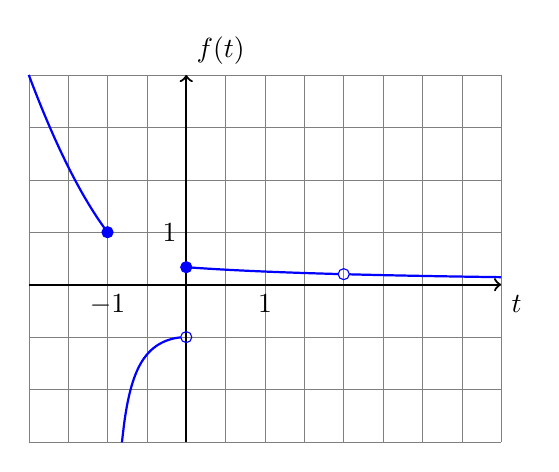
\begin{tikzpicture}
[
	closedpt/.style={circle,draw,fill,inner sep=0pt,minimum size=4pt},
	openpt/.style={circle,draw,inner sep=0pt,minimum size=4pt},
	yscale=0.666
]

	% grid
	\foreach \x in {-2,-1.5,-1,...,4} {
		\draw[very thin,gray] (\x,\ymin) -- (\x,\ymax);
	}
	\foreach \y in {-3,-2,...,4} {
		\draw[very thin,gray] (\xmin,\y) -- (\xmax,\y);
	}

	% label grid
	\foreach \x in {-1,1} {
		\node[below] at (\x,0) {$\x$};
	}
	\foreach \y in {1} {
		\node[left] at (0,\y) {$\y$};
	}

	% axes
	\draw[->,thick] (\xmin,0) -- (\xmax,0) node[below right] {$t$};
	\draw[->,thick] (0,\ymin) -- (0,\ymax) node[above right] {$f(t)$};

	% parabolic portion
	\draw[thick, blue, domain=-2:-1,smooth] plot (\x,{\x * \x});
	\node[blue,closedpt] at (-1,1) {};

	% reciprocal power portion
	\draw[thick, blue, domain=-0.817:-0.07,smooth] plot (\x,{1 / (\x * \x - 1)});
	\node[blue,openpt] at (0,-1) {};

	% rational function, simplified to reciprocal function
	\draw[thick, blue, domain=0:1.93,smooth] plot (\x,{1 / (\x + 3)});
	\draw[thick, blue, domain=2.07:4,smooth] plot (\x,{1 / (\x + 3)});
	\node[blue,closedpt] at (0,0.333) {};
	\node[blue,openpt] at (2,0.2) {};

\end{tikzpicture}
